%20 min preso!
\documentclass[xcolor=table]{beamer}
\usepackage{beamerthemesplit}
\usepackage{wrapfig}
\usetheme{SPbGU}
\usepackage{pdfpages}
\usepackage{amsmath}
\usepackage{cmap}
\usepackage[T2A]{fontenc}
\usepackage[utf8]{inputenc}
\usepackage[english]{babel}
\usepackage{indentfirst}
\usepackage{amsmath}
\usepackage{tikz}
\usepackage{multirow}
\usepackage[noend]{algpseudocode}
\usepackage{algorithm}
\usepackage{algorithmicx}
\usepackage{fancyvrb}
\usetikzlibrary{calc}
\usetikzlibrary{shapes,arrows}

\usepackage{tabularx}
\newcolumntype{Y}{>{\raggedleft\arraybackslash}X}


\newtheorem{mytheorem}{Theorem}
\renewcommand{\thealgorithm}{}

\newcommand{\tikzmark}[1]{\tikz[overlay,remember picture] \node (#1) {};}
\def\Put(#1,#2)#3{\leavevmode\makebox(0,0){\put(#1,#2){#3}}}

\beamertemplatenavigationsymbolsempty

\title[DNN + Formal Grammars]{The Composition of Dense Neural Networks and Formal~Grammars for Secondary Structure Analysis}
%\subtitle[YaccConstructor]{Parsing techniques for graph analysis}
% То, что в квадратных скобках, отображается в левом нижнем углу.
\institute[JetBrains Research]{
JetBrains Research, Programming Languages and Tools Lab  \\
Saint Petersburg University
}

% То, что в квадратных скобках, отображается в левом нижнем углу.
\author[Semyon Grigorev]{Polina Lunina, \textbf{Semyon Grigorev}}

\date{Febrary !!!, 2019}

\begin{document}
{
\begin{frame}[fragile]
  \begin{table}
  \centering
  \begin{tabularx}{\linewidth}{YcX}
    
\includegraphics[height=1.5cm]{pictures/jetbrainsResearch.pdf} \hfill
    & \begin{minipage}[t]{0.3\textwidth}\center \vspace{-1cm}  BIOINFORMATICS 2019
      \end{minipage}
    & \hfill 
\includegraphics[height=1.5cm]{pictures/SPbGU_Logo.png}
  \end{tabularx}
  \end{table}
  \titlepage
\end{frame}
}

\begin{frame} \frametitle{Sequences Analysis}

\begin{itemize}
   \item Sequences classification
   \item Subsequences seqrch
   \item \dots
\end{itemize}
\pause
\begin{minipage}[t]{0.48\textwidth}

\textbf{Problem: high variability of data}
\begin{itemize}
   \item Mutattions
   \item Different kinds of noice
   \item \dots
\end{itemize}
\pause
\textbf{We need probabilistic approaches}
\end{minipage}
\pause
~
\begin{minipage}[t]{0.48\textwidth}
\textbf{Level of abstraction}
\begin{itemize}
   \item Plain text
   \item Secondary structure
   \item 3D structure
\end{itemize}
\pause
\textbf{We should handle secondary structure}
\end{minipage}

\end{frame}


\begin{frame} \frametitle{Probabilistic approaches}

\begin{itemize}
  \item Hidden Markov's Models (HMM's)
  \item Probabilistic grammars
  \item Covariation Models (CM's)
  \item Artificial neural networks
\end{itemize}

\end{frame}


\begin{frame} \frametitle{Our receip: Parsing + DNN}

\begin{itemize}
  \item Idea: not secondary structure modelling, but features extraction!
\end{itemize}

\end{frame}


\begin{frame} \frametitle{Our receip: Parsing + DNN}

\begin{itemize}
  \item Idea description. Figure
\end{itemize}

\end{frame}

\begin{frame}[fragile] \frametitle{Grammar}
\begin{verbatim}
s1: stem<s0>
any_str : any_smb*[2..10]
any_smb: A | T | C | G
s0: any_str | any_str stem<s0> s0
stem1<s>:               \\ stem of height exactly 1
      A s T | G s C | T s A | C s G
stem2<s>:               \\ stem of height exactly 2
      stem1< stem1<s> >
stem<s>:                \\ stem of height 3 or more
      A stem<s> T
    | T stem<s> A
    | C stem<s> G
    | G stem<s> C
    | stem1< stem2<s> >
\end{verbatim}
\pause
\only<1-2>{\tikz[overlay,remember picture]{\draw[draw=red,thick,double,fill opacity=0.2] ($(-0.2,5.6)$) rectangle ($(12,4.6)$);}}
\only<3-3>{\tikz[overlay,remember picture]{\draw[draw=red,thick,double,fill opacity=0.2] ($(-0.2,4.6)$) rectangle ($(12,3.6)$);}}
\only<4-4>{\tikz[overlay,remember picture]{\draw[draw=red,thick,double,fill opacity=0.2] ($(-0.2,3.6)$) rectangle ($(12,0.6)$);}}
\end{frame}

\begin{frame}[fragile] \frametitle{Example 1: Stem}
\centering
 $\omega_1=$ \texttt{CCCCATTGCCAAGGACCCCACCTTGGCAATCCC}
\vspace{1cm}

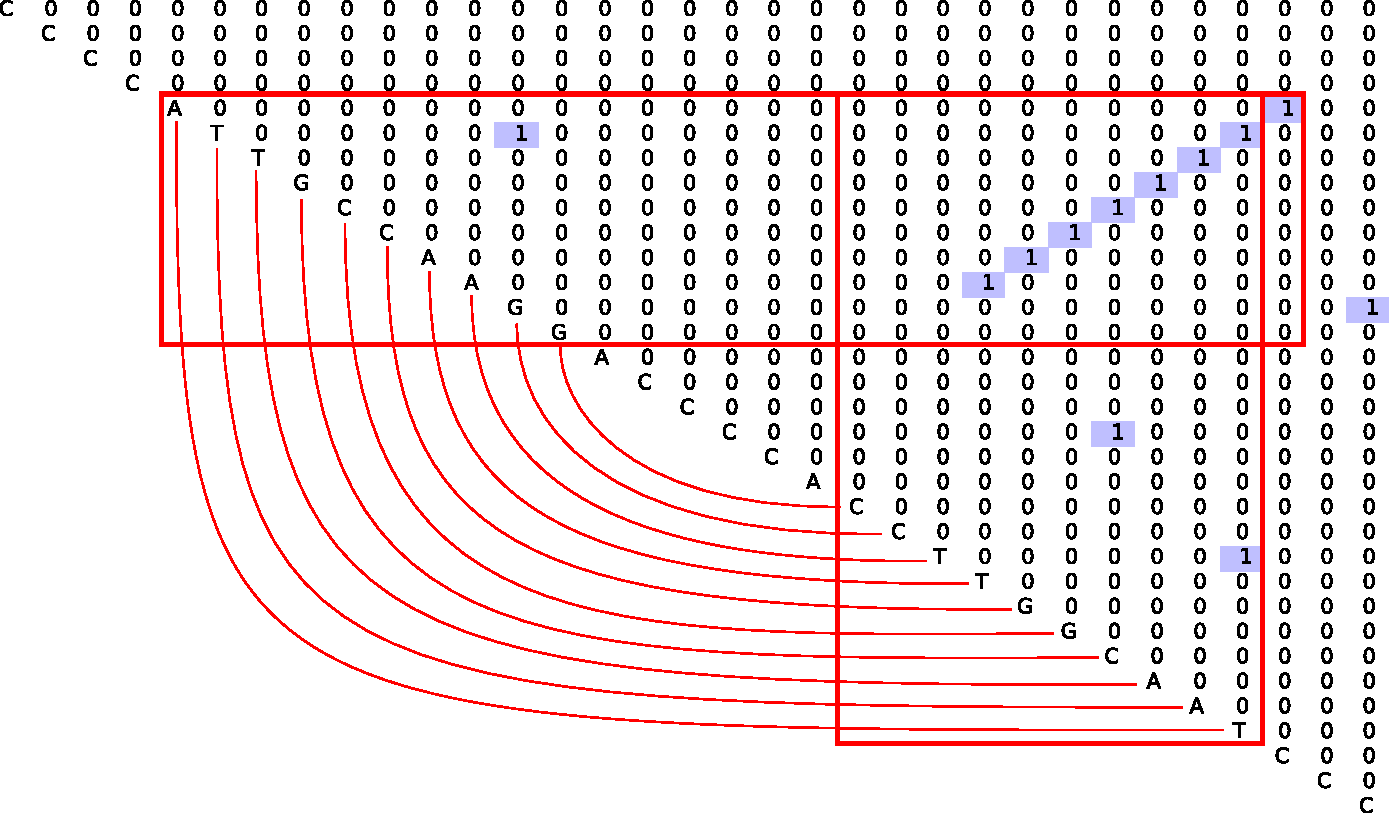
\includegraphics[width=.8\textwidth]{pictures/4.pdf}

\end{frame}

\begin{frame}[fragile] \frametitle{Example 2: Pseudoknot}
\centering
 $\omega_2=$ \texttt{CCACTTACCTATGACCTAAGTCCTCATACC}
\vspace{1cm}

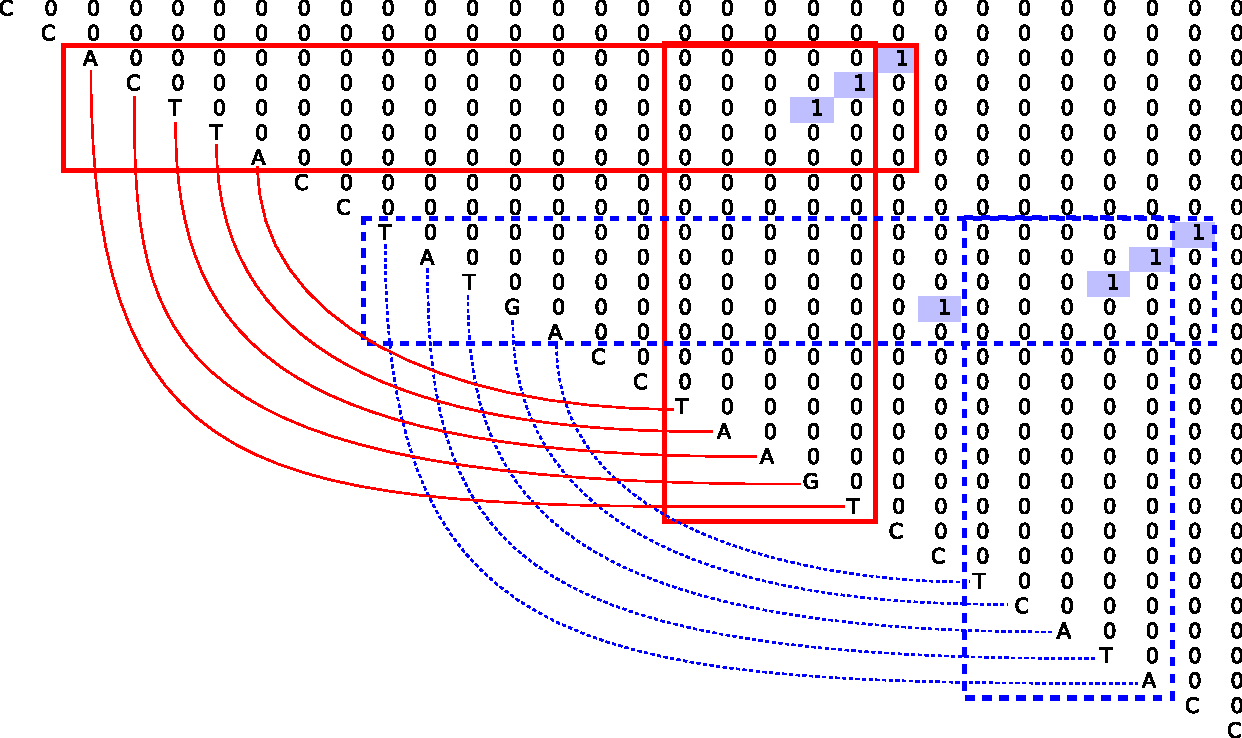
\includegraphics[width=.8\textwidth]{pictures/5.pdf}

\end{frame}


\begin{frame}[fragile] \frametitle{Example 3: real tRNA}
\centering
 $\omega_3=$ \texttt{CAGGGCATAACCTAGCCCAACCTTGCCAAGG\\TTGGGGTCGAGGGTTCGAATCCCTTCGCCCGCTCCA}\footnote{\tiny{Novosphingobium aromaticivorans from GtRNAdb.}}
\vspace{0.5cm}

Predicted secondary structures\footnote{\tiny{Results are given by using the \href{http://rna.urmc.rochester.edu/RNAstructureWeb/Servers/Fold/Fold.html}{Fold Web Server with default settings}.}}

\begin{minipage}[t]{0.49\textwidth}
\centering
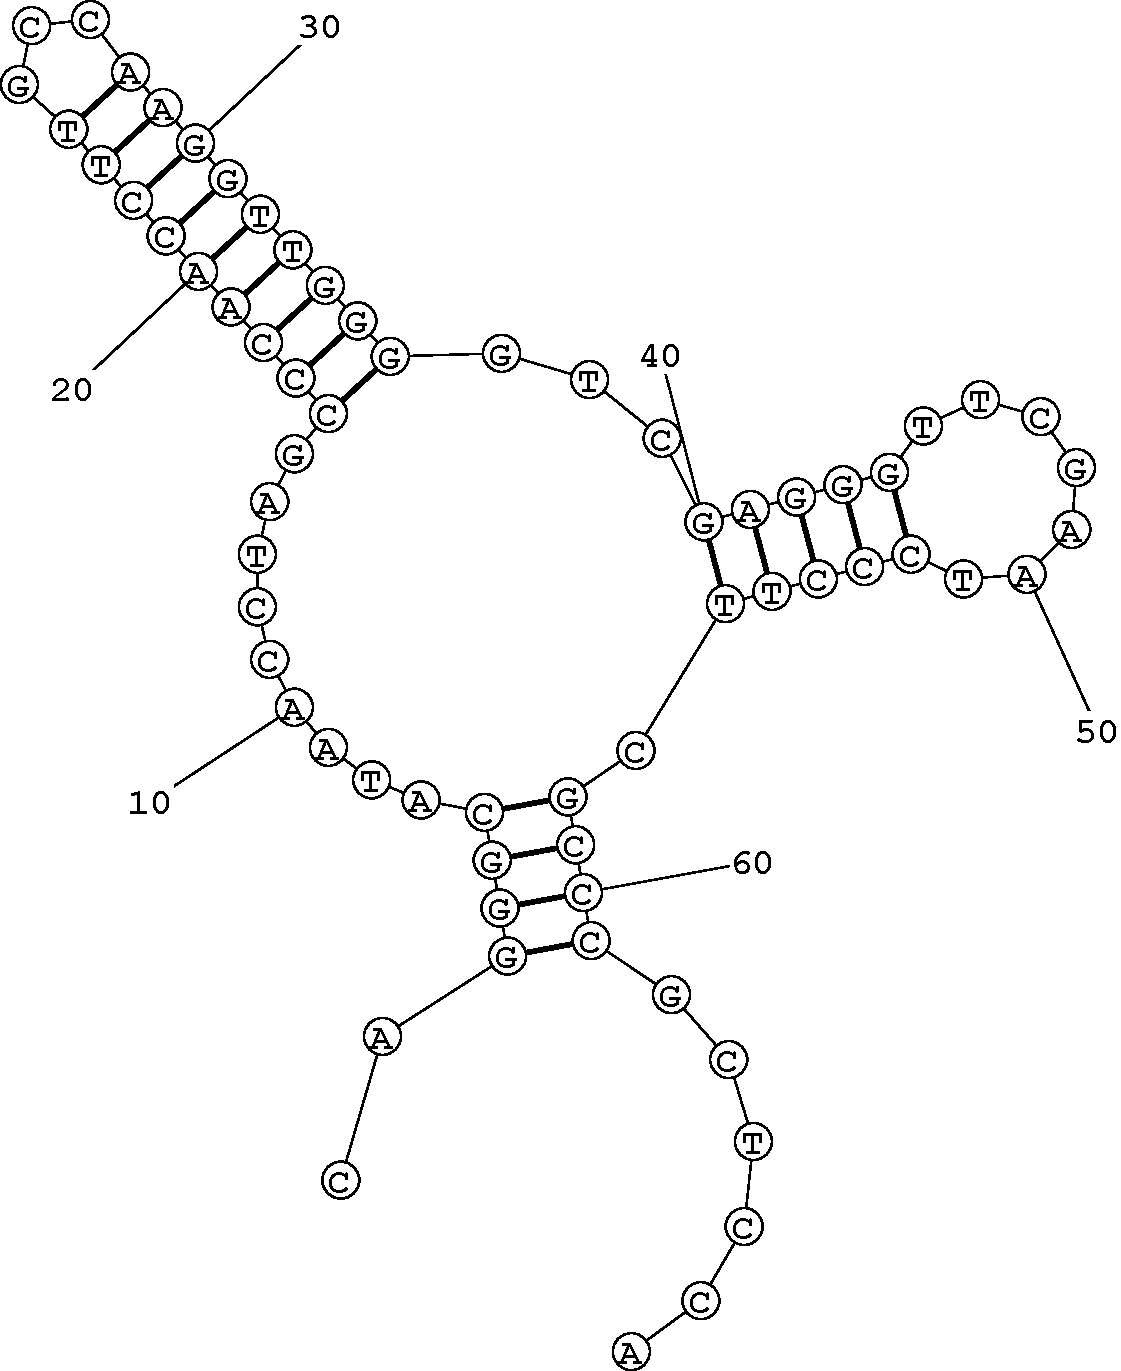
\includegraphics[width=.70\textwidth]{pictures/Fold1.pdf}
\end{minipage}
\begin{minipage}[t]{0.49\textwidth}
\centering
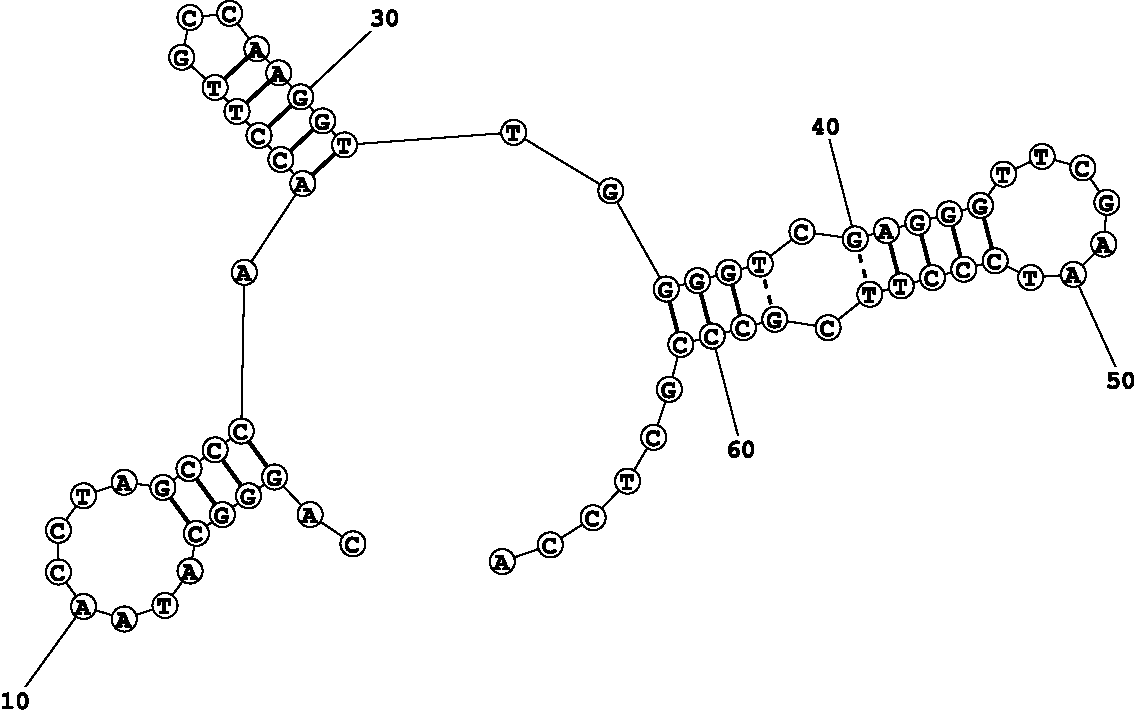
\includegraphics[width=.96\textwidth]{pictures/Fold2.pdf}
%\vspace{1cm}
%\vfill
\end{minipage}

\end{frame}

\begin{frame}[fragile] \frametitle{Example 3: real tRNA}
\centering
%\only<1-8>{
\tikzmark{an}{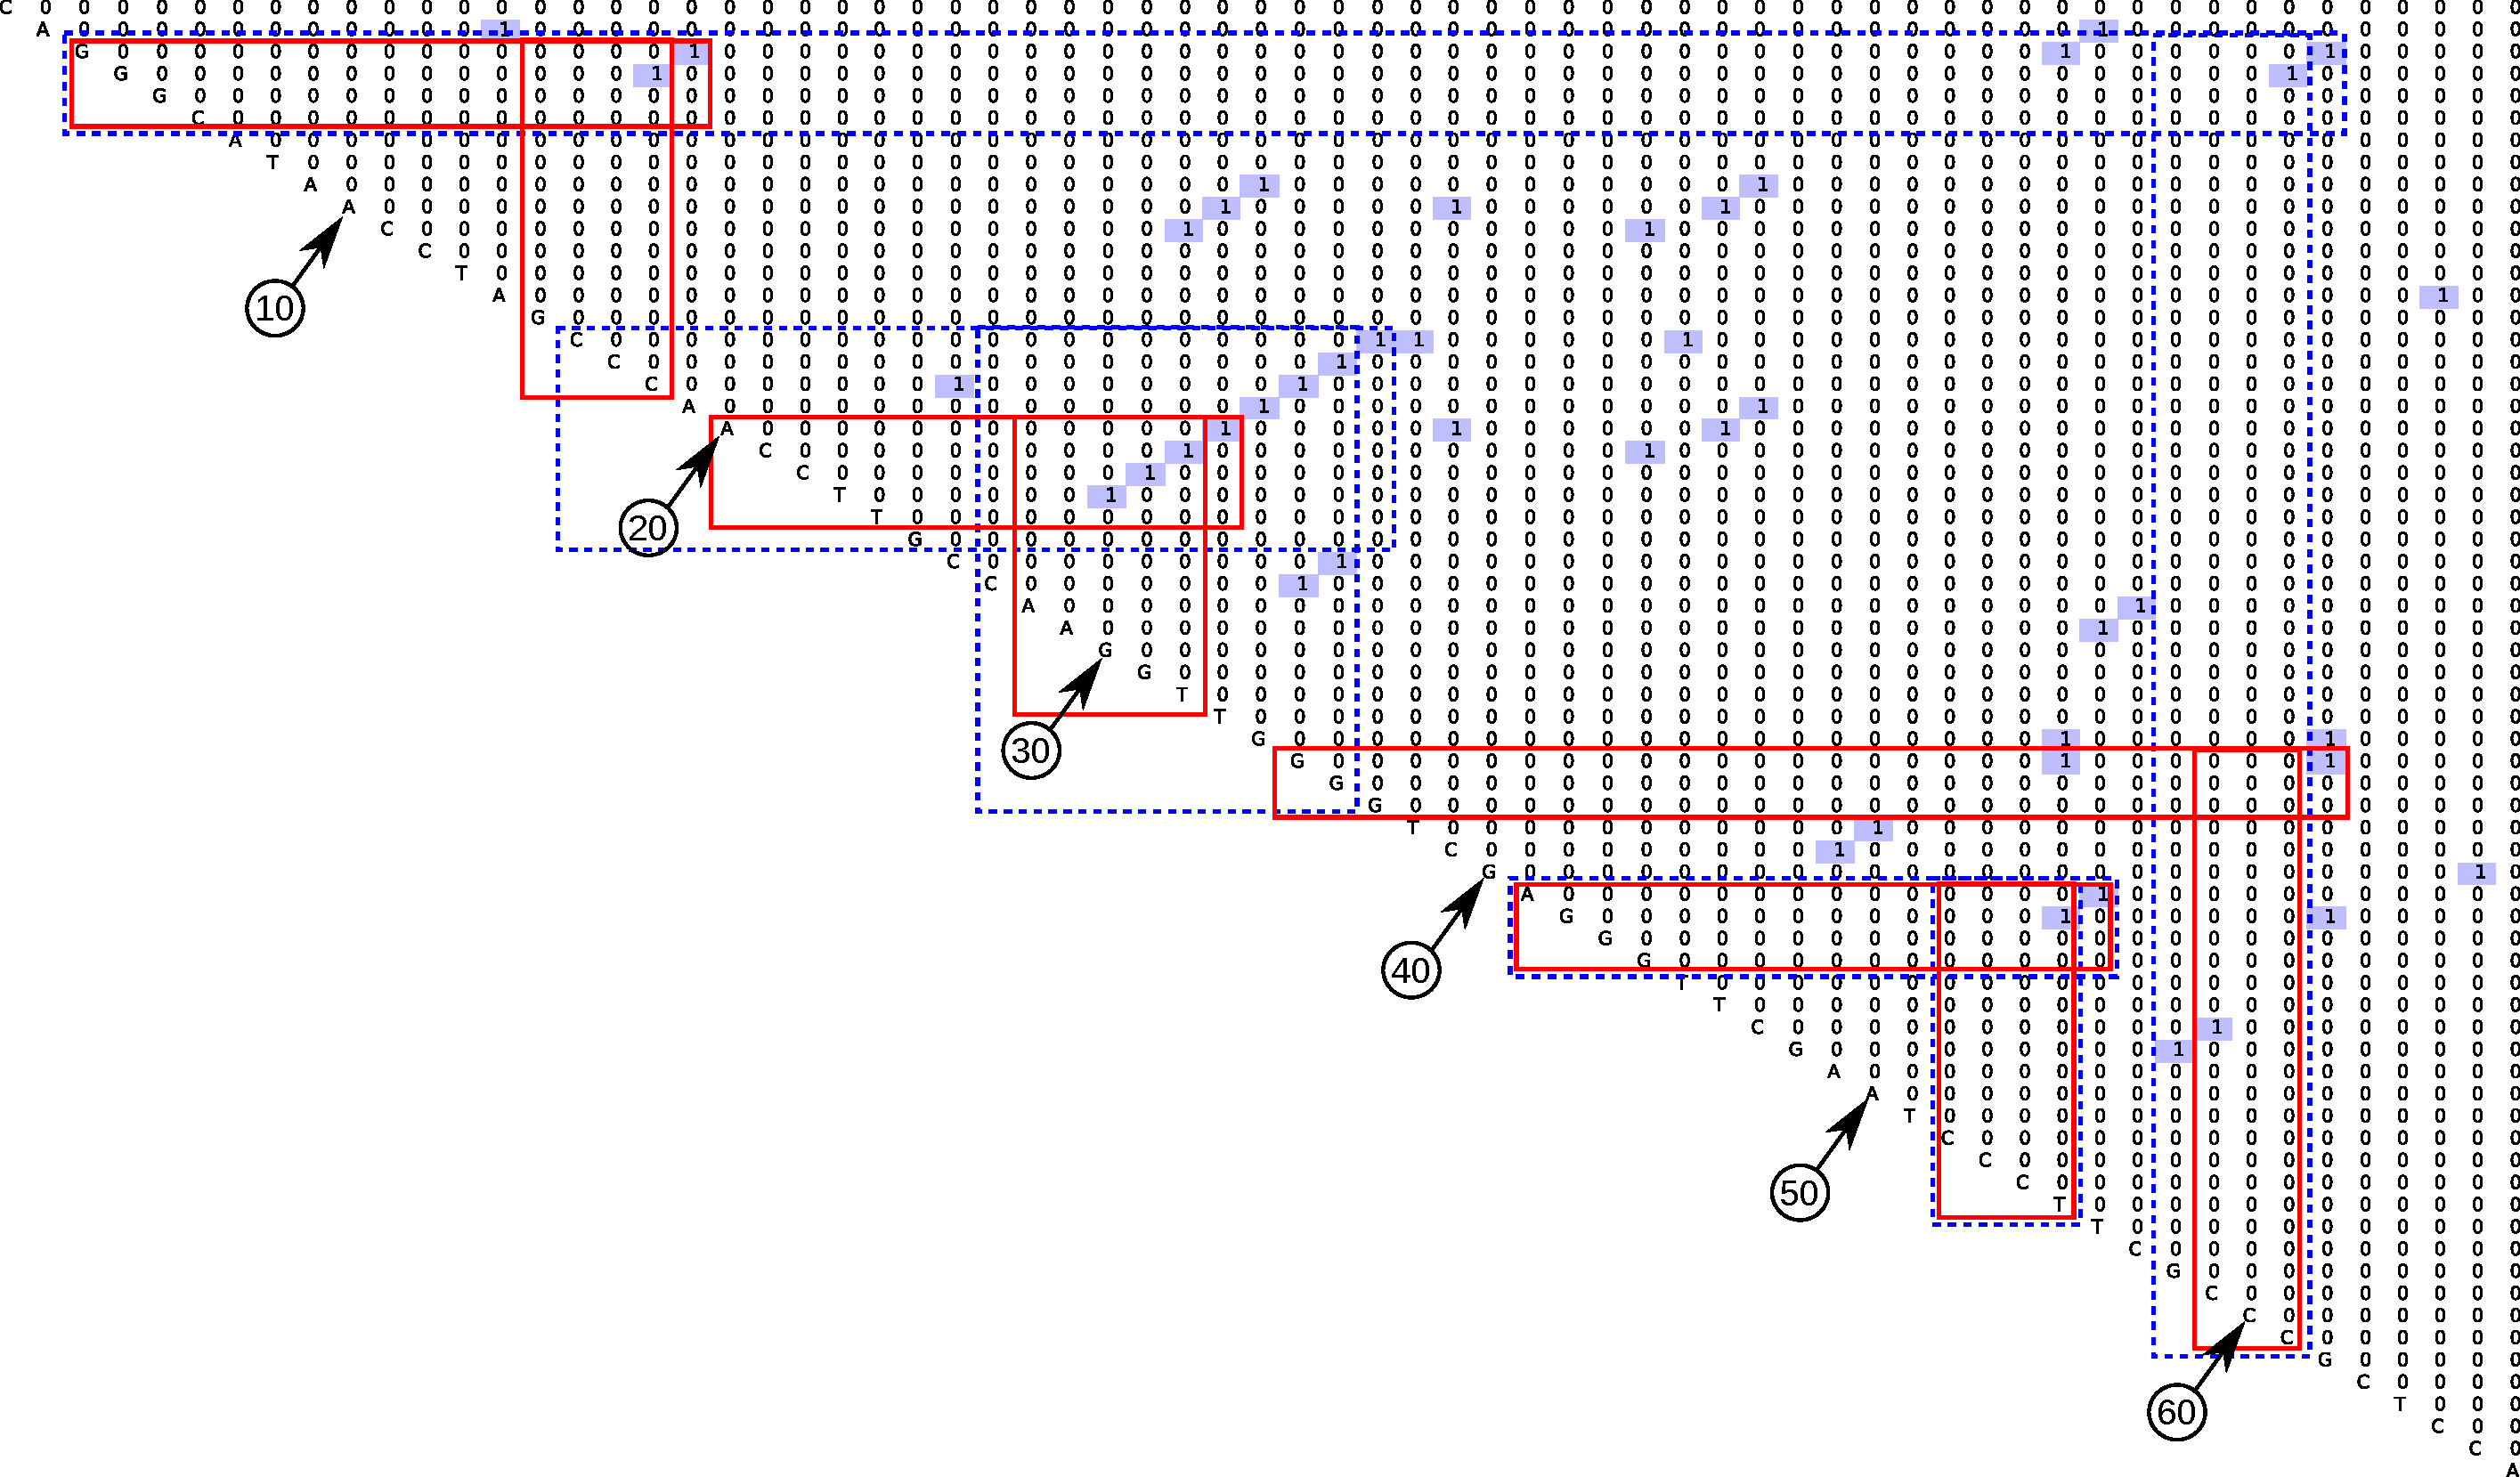
\includegraphics[width=\textwidth]{pictures/0m.pdf}}
%}
\onslide<2-3>{\Put(-175,150){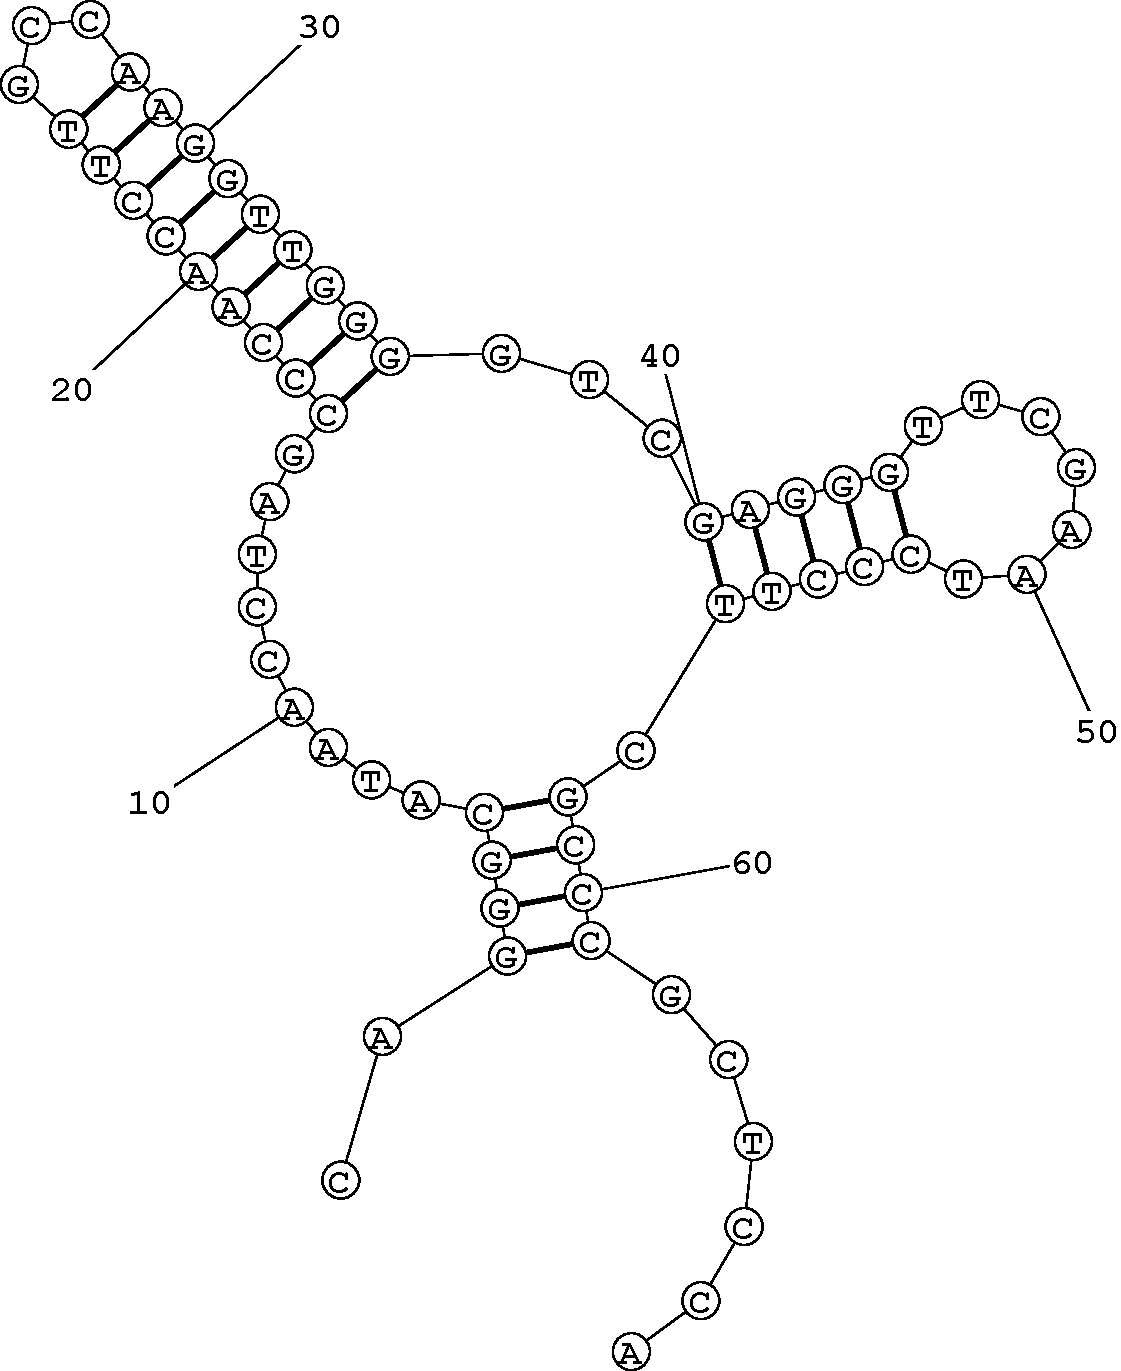
\includegraphics[height=6cm]{pictures/Fold1.pdf}}}
\onslide<3-3,7>{
\tikz[overlay,remember picture]{
\draw[draw=blue,thick,fill opacity=0.2] ($(an) + (0.28,6.885)$) rectangle ($(an) + (11.22,6.415)$);
\draw[draw=blue,thick,fill opacity=0.2] ($(an) + (10.3,6.885)$) rectangle ($(an) + (11.025,0.57)$);

\draw[draw=blue,thick,fill opacity=0.2] ($(an) + (2.65,5.49)$) rectangle ($(an) + (6.68,4.42)$);
\draw[draw=blue,thick,fill opacity=0.2] ($(an) + (4.65,5.49)$) rectangle ($(an) + (6.46,3.2)$);

\draw[draw=blue,thick,fill opacity=0.2] ($(an) + (7.2,2.85)$) rectangle ($(an) + (10.12,2.4)$);
\draw[draw=blue,thick,fill opacity=0.2] ($(an) + (9.23,2.85)$) rectangle ($(an) + (9.95,1.2)$);
}
}

\onslide<5-6>{\Put(-10,130){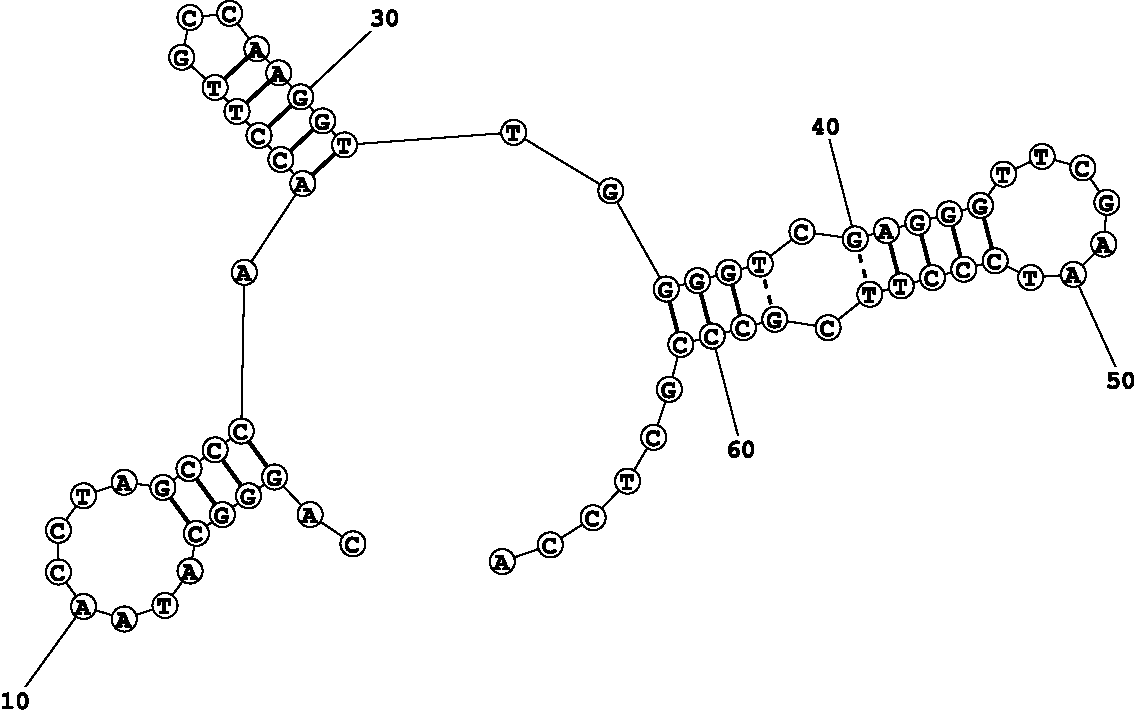
\includegraphics[height=4.3cm]{pictures/Fold2.pdf}}}
\onslide<6-7>{
\tikz[overlay,remember picture]{

\draw[draw=red,thick,fill opacity=0.2] ($(an) + (0.31,6.86)$) rectangle ($(an) + (3.4,6.44)$);
\draw[draw=red,thick,fill opacity=0.2] ($(an) + (2.5,6.86)$) rectangle ($(an) + (3.2,5.1)$);

\draw[draw=red,thick,fill opacity=0.2] ($(an) + (3.4,5.06)$) rectangle ($(an) + (5.95,4.535)$);
\draw[draw=red,thick,fill opacity=0.2] ($(an) + (4.83,5.06)$) rectangle ($(an) + (5.73,3.6)$);

\draw[draw=red,thick,fill opacity=0.2] ($(an) + (6.1,3.47)$) rectangle ($(an) + (11.2,3.15)$);
\draw[draw=red,thick,fill opacity=0.2] ($(an) + (10.5,3.47)$) rectangle ($(an) + (11,0.6)$);

\draw[draw=red,thick,fill opacity=0.2] ($(an) + (7.2,2.85)$) rectangle ($(an) + (10.12,2.4)$);
\draw[draw=red,thick,fill opacity=0.2] ($(an) + (9.23,2.85)$) rectangle ($(an) + (9.95,1.2)$);
}
}
\end{frame}

\begin{frame} \frametitle{Summary}

\begin{itemize}
  \item Parser is a features extructor
  \item All possible foldings
  \item Grammar is a varaible parameter
  \item It is possible to detect features which is not expressable in language class which in use
\end{itemize}

\end{frame}

\begin{frame} \frametitle{Artificial Neural Networks}
We use dence neural network
\begin{itemize}
  \item Problem: fixed size of input. Special simbol
  \item agressive dropout and batch normalization
  \item !!!
\end{itemize}

\end{frame}

\begin{frame} \frametitle{Evaluation}
\begin{itemize}
 \item 16s rRNA detection
 \begin{itemize}
  \item Type provider is a \textbf{function which constructs type}
 \end{itemize}
\pause
\item tRNA classification
\begin{itemize}
 \item Type provider is a \textbf{function which constructs type}
\end{itemize}
\end{itemize}

\end{frame}

\begin{frame} \frametitle{Future work}

\begin{itemize}
 \item DNN without parsing
 \item Other types of neural networks
 \item More !!! Evaluation
 \item Comprison with other tools
\end{itemize}

\end{frame}

\begin{frame}
%\transwipe[direction=90]
\frametitle{Contact Information}
\begin{itemize}
  \item Semyon Grigorev:
    \begin{itemize}
      \item \href{mailto:s.v.grigoriev@spbu.ru}{s.v.grigoriev@spbu.ru}
      \item \href{mailto:Semen.Grigorev@jetbrains.com}{Semen.Grigorev@jetbrains.com}
    \end{itemize}
  \item Polind Lunina:
  \begin{itemize}
    \item  \href{mailto:lunina_polina@mail.ru}{lunina\_polina@mail.ru}
  \end{itemize}
  \item Trained models:
\end{itemize}
\vspace{2cm}
\pause
\center{\huge{Thanks!}}
\end{frame}
\end{document}
